\documentclass[UTF8]{article}
\usepackage{graphicx}
\usepackage{subfigure}
\usepackage{amsmath}
\usepackage{makecell}
\usepackage[utf8]{inputenc}
\usepackage[space]{ctex} %中文包
\usepackage{listings} %放代码
\usepackage{xcolor} %代码着色宏包
\usepackage{CJK} %显示中文宏包
\usepackage{float}
\usepackage{makecell}
\usepackage{diagbox}
\usepackage{bm}
\usepackage{ulem} 
\usepackage{amssymb}
\usepackage{soul}
\usepackage{color}
\usepackage{geometry}
\usepackage{fancybox} %花里胡哨的盒子
\usepackage{xhfill} %填充包, 可画分割线 https://www.latexstudio.net/archives/8245
\usepackage{multicol} %多栏包
\usepackage{enumerate} %可以方便地自定义枚举标题
\usepackage{multirow} %表格中多行单元格合并
\usepackage{wasysym} %可以使用wasysym里的一堆奇奇怪怪的符号
\usepackage{tikz}
\usepackage{tikZ-timing}
\usetikzlibrary{shadows} % 阴影支持\AddEnumerateCounter{\chinese}{\chinese}{}

\geometry{left = 1cm, right = 1cm, top=1cm, bottom=1cm}

\definecolor{mygreen}{rgb}{0,0.6,0}
\definecolor{mygray}{rgb}{0.5,0.5,0.5}
\definecolor{mymauve}{rgb}{0.58,0,0.82}
\lstset{
	backgroundcolor=\color{white}, 
	%\tiny < \scriptsize < \footnotesize < \small < \normalsize < \large < \Large < \LARGE < \huge < \Huge
	basicstyle = \footnotesize,       
	breakatwhitespace = false,        
	breaklines = true,                 
	captionpos = b,                    
	commentstyle = \color{mygreen}\bfseries,
	extendedchars = false,
	frame = shadowbox, 
	framerule=0.5pt,
	keepspaces=true,
	keywordstyle=\color{blue}\bfseries, % keyword style
	language = C++,                     % the language of code
	otherkeywords={string}, 
	numbers=left, 
	numbersep=5pt,
	numberstyle=\tiny\color{mygray},
	rulecolor=\color{black},         
	showspaces=false,  
	showstringspaces=false, 
	showtabs=false,    
	stepnumber=1,         
	stringstyle=\color{mymauve},        % string literal style
	tabsize=4,          
	title=\lstname           
}

%\sum\nolimits_{j=1}^{M}   上下标位于求和符号的水平右端,
%\sum\limits_{j=1}^{M}   上下标位于求和符号的上下处,
%\sum_{j=1}^{M}  对上下标位置没有设定,会随公式所处环境自动调整。

%%%%%%%%%%%%%画图包%%%%%%%%%%%%%
\usepackage{tikz}
%%%%%%%%%%%%%好看的矩形%%%%%%%%%%%%%
\tikzset{
  rect1/.style = {
    shape = rectangle,% 指定样式
    minimum height=2cm,% 最小高度
    minimum width=4cm,% 最小宽度
    align = center,% 文字居中
    drop shadow,% 阴影
  }
}
%%%%%%%%%%%%%画图背景包%%%%%%%%%%%%%
\usetikzlibrary{backgrounds}

%%%%%%%%%%%%%在tikz中画一个顶点%%%%%%%%%%%%%
%%%%%%%%%%%%%#1:node名称%%%%%%%%%%%%%
%%%%%%%%%%%%%#2:位置%%%%%%%%%%%%%
%%%%%%%%%%%%%#3:标签%%%%%%%%%%%%%
\newcommand{\newVertex}[3]{\node[circle, draw=black, line width=1pt, scale=0.8] (#1) at #2{#3}}
%%%%%%%%%%%%%在tikz中画一条边%%%%%%%%%%%%%
\newcommand{\newEdge}[2]{\draw [black,very thick](#1)--(#2)}
%%%%%%%%%%%%%在tikz中放一个标签%%%%%%%%%%%%%
%%%%%%%%%%%%%#1:名称%%%%%%%%%%%%%
%%%%%%%%%%%%%#2:位置%%%%%%%%%%%%%
%%%%%%%%%%%%%#3:标签内容%%%%%%%%%%%%%
\newcommand{\newLabel}[3]{\node[line width=1pt] (#1) at #2{#3}}

%%%%%%%%%%%%%强制跳过一行%%%%%%%%%%%%%
\newcommand{\jumpLine} {\hspace*{\fill} \par}
%%%%%%%%%%%%%关键点指令,可用itemise替代%%%%%%%%%%%%%
\newcommand{\average}[1]{\left\langle #1\right\rangle }
%%%%%%%%%%%%%表格内嵌套表格%%%%%%%%%%%%%
\newcommand{\keypoint}[2]{$\bullet$\textbf{#1}\quad#2\par}
%%%%%%%%%%%%%<T>平均值表示%%%%%%%%%%%%%
\newcommand{\tabincell}[2]{\begin{tabular}{@{}#1@{}}#2\end{tabular}}%放在导言区
%%%%%%%%%%%%%大黑点item头%%%%%%%%%%%%%
\newcommand{\itemblt}{\item[$\bullet$]}
%%%%%%%%%%%%%大圈item头%%%%%%%%%%%%%
\newcommand{\itemc}{\item[$\circ$]}
%%%%%%%%%%%%%大星星item头%%%%%%%%%%%%%
\newcommand{\itembs}{\item[$\bigstar$]}
%%%%%%%%%%%%%右▷item头%%%%%%%%%%%%%
\newcommand{\itemrhd}{\item[$\rhd$]}
%%%%%%%%%%%%%定义为%%%%%%%%%%%%%
\newcommand{\defas}{=_{df}}
%%%%%%%%%%%%%蕴含%%%%%%%%%%%%%
\newcommand{\imp}{\rightarrow}

%%%%%%%%%%%%%双线分割线%%%%%%%%%%%%%
\newcommand*{\doublerule}{\hrule width \hsize height 1pt \kern 0.5mm \hrule width \hsize height 2pt}
%%%%%%%%%%%%%双线中间可加东西的分割线%%%%%%%%%%%%%
\newcommand\doublerulefill{\leavevmode\leaders\vbox{\hrule width .1pt\kern1pt\hrule}\hfill\kern0pt }
%%%%%%%%%%%%%左大括号%%%%%%%%%%%%%
\newcommand{\leftbig}[1]{\left\{\begin{array}{l}#1\end{array}\right.}
%%%%%%%%%%%%%矩阵%%%%%%%%%%%%%
\newcommand{\mat}[2]{\left[\begin{array}{#1}#2\end{array}\right]}
%%%%%%%%%%%%%可换行圆角文本框%%%%%%%%%%%%%

\newcommand{\ovalboxn}[1]{\ovalbox{\tabincell{l}{#1}}}
%%%%%%%%%%%%%设置section的counter, 使从0开始%%%%%%%%%%%%%
\setcounter{section}{-1}

\title{\begin{Huge}中国科学技术大学\end{Huge}\\\begin{Large}2016-2017学年第二学期考试试卷\end{Large}}
\date{}

\begin{document}
\maketitle
\begin{enumerate}[I]
\item 简答题
	\begin{enumerate}[1]
	\item 现代化计算机优化冯诺依曼结构\\
	\ovalbox{是说以存储器为中心, 而不再以CPU为中心吗?}
	\item 指令类型\&寻址方式\\
		就MIPS而言, 指令类型可以按照多种方式分类
		\begin{itemize}
		\item 按照指令格式有R类I类J类等
		\item 按照指令功能有运算,分支,跳转, 访存等
		\end{itemize}
		寻址方式的话则有R类的寄存器寻址, I类的立即寻址(直接是立即数而不是地址), 基址寻址, 相对寻址(访存等), J类的伪直接寻址
	\item 中断系统组成\\
		中断系统由以下部件组成
		\begin{itemize}
		\item 硬件上需要程序状态字中的中断使能标志, 需要中断请求标志等寄存器(INTR,INTA).
		\item 指令上需要实现中断隐指令以保护现场, 需要专用寄存器存储当前PC或借助存储器
		\item 断点/现场保存需要存在存储器里
		\item 中断服务程序(ISR入口有向量方式和非向量方式, 都应预先在存储器里设置好)和中断判优器(如果是硬件实现的话)
		\end{itemize}
	\item 总线同步异步时序图\\
	同步读示意(写类似):
	\begin{tikzpicture}
	\timing [
	yscale=2.0,
	timing/wscale=3.0,
	timing/inline 
	node/.style={rectangle,below left,font=\sffamily}
	] at (0,0)
	{
	2H 2L N[above]{Addr} 3L H
	};
	\timing [
	yscale=2.0,
	timing/wscale=3.0,
	timing/inline 
	node/.style={rectangle,below left,font=\sffamily}
	] at (0,-1)
	{
	3H 1.5L N[above]{Read} 1.5L 2H
	};
	\timing [
	yscale=2.0,
	timing/wscale=3.0,
	timing/inline 
	node/.style={rectangle,below left,font=\sffamily}
	] at (0,-2)
	{
	5H 0.5L N[above]{Data} 0.5L 2H
	};
	\end{tikzpicture}\\
	异步有不互锁, 半互锁, 全互锁, 分别是123次交流
	\item 快表和慢表的作用
		\begin{itemize}
		\item 快表可以加快对页表内容的访问. 具体而言就是快表能够避免对存储器的二次访问, 将热点页号保存在快表中, 并以很高性能的硬件实现完成.
		\item 都说慢了还能有作用?页表的作用: 页表解决了虚拟内存机制的地址映射问题.
		\end{itemize}
	\item 示意图表示指令周期,机器周期,访存周期,总线周期,DMA周期
		\begin{itemize}
		\item 指令周期: 取决于CPU设计(单周期多周期流水线), 应该是机器周期的倍数
		\item 访存周期: 应该是在指令周期之间的我猜?这里涉及到了访存的多级Cache, 所以可能会要多个周期来完成.
		\item 总线周期: 包括申请分配阶段(总线仲裁), 寻址阶段, 传送阶段, 结束阶段(让出总线使用权). 大概就是画一下同步(包括读写)异步(不互锁, 半互锁, 全互锁)半同步(除了有等待线都是同步的)和分离式(拿到总线后发地址和命令,然后放弃总线; 模块准备好数据后第二阶段再申请总线)?
		\item DMA周期: 发命令之后就等它做完引起中断处理后事了. 但中间涉及到周期窃取,交替访存等(这是由于DMA和CPU可能同时需要访问存储器)
		\end{itemize}
	\item CPU设计步骤\\
		指令集、 单周期、 多周期、 流水线、 数据通路、 控制信号、 状态机(抄xyy的)
	\item PC和手机的区别\\
		随便回答hhh
	\end{enumerate}
\item 综合题
	\begin{enumerate}[1]
	\item 用4位Booth算法计算3*4(7分)\\
		没学过
	\item Cache直接映射, 判断hit/miss(8分)\\
		直接映射就是Cache块号=主存块号 mod Cache块数的那种.
		顺便: 
		\begin{itemize}
		\item 全相联映射就是直接存块号+块内地址的, 主存里任何一块都可以放在Cache里任何一块. Cache里有相联存储器判断块号在不在.
		\item 组相联是直接映射里套全相联
		\end{itemize}
	\item disk/DMA controller 作用, 工作方式
		作用就是传输不用CPU, CPU可以做别的事. 工作方式就描述一遍读写过程.
	\item 计算存储器单个芯片全部以及总容量, 位数\\
		?
	\item abs instruction : why mips don’t have?, if have, what format?
		大概是太简单了吧, x86和RISC-V的整数算逻都没有abs指令, 只有float有.
	\item pipeline
		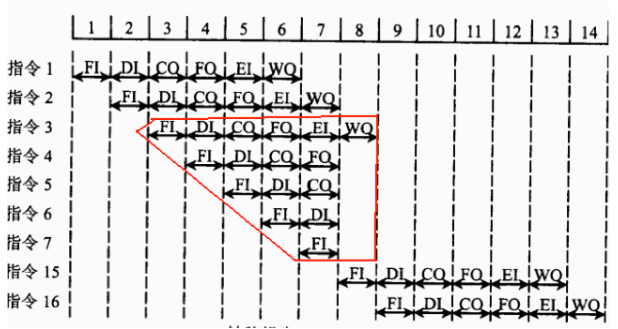
\includegraphics[scale=0.5]{pipeline.png}
		\begin{enumerate}[i]
		\item 跳转指令是:\underline{ 指令3}
		\item 延迟槽可以插入\underline{4}条指令
		\item 为减少流水线损失可以采取哪些措施?
			\begin{itemize}
			\item 分支预测
			\item 提前beq
			\item 流水线深度改浅
			\end{itemize}
		\end{enumerate}
	\item 指令执行
		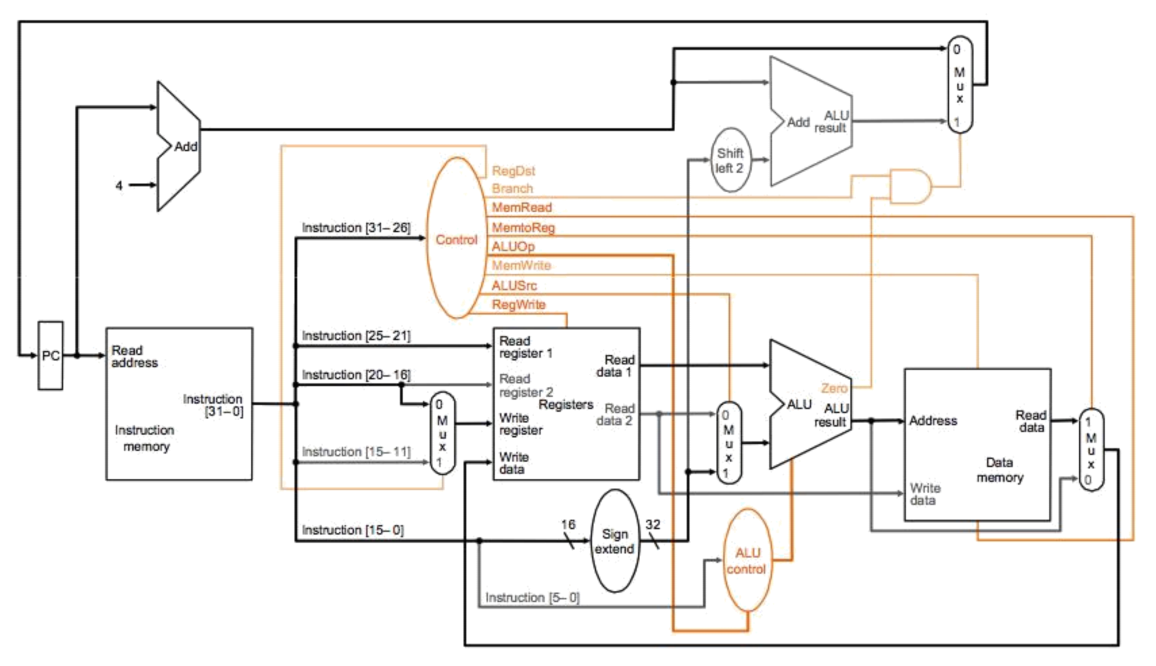
\includegraphics[scale=0.5]{cpu.png}
		\begin{enumerate}[i]
		\item and,sw执行过程?
		\item 执行中控制信号?
		\item 单周期, 则指令周期长度?
	
	\end{enumerate}
\end{enumerate}

\end{document}